% small.tex
\documentclass{beamer}
%include polycode.fmt
\usepackage{xcolor}
\usepackage{media9}
\usepackage{tikz}
\usetikzlibrary{patterns}
\usepackage{pgfplots}
\usepackage[normalem]{ulem}
\usepackage{color, colortbl}
\usepackage{tikz}
\usetikzlibrary{arrows,%
                shapes,positioning}
\usetikzlibrary{trees}
\usetikzlibrary{shapes}
\definecolor{green}{rgb}{0,1,0}
\definecolor{navyblue}{rgb}{0.2,0.2,0.7}
\usetheme{Antibes}
\useoutertheme[subsection=false]{miniframes}
\usenavigationsymbolstemplate{}
\newsavebox\MBox
\newcommand\Cline[2][red]{{\sbox\MBox{$#2$}%
  \rlap{\usebox\MBox}\color{#1}\rule[-1.2\dp\MBox]{\wd\MBox}{0.5pt}}}
  
\title{Monadic Functional Reactive Programming}
\author{Atze van der Ploeg}
\institute{
Centrum Wiskunde \& Informatica, Amsterdam, The Netherlands}

\newcommand{\dfcode}[1]{\begin{flalign*}\vspace{-0.35cm}#1\vspace{-0.35cm}\end{flalign*}}
\newcommand{\mul}{\!\times\!}
% \date{\today}

\newcommand{\beginbackup}{
   \newcounter{framenumbervorappendix}
   \setcounter{framenumbervorappendix}{\value{framenumber}}
}

\newcommand{\frameofframes}{/}
\newcommand{\setframeofframes}[1]{\renewcommand{\frameofframes}{#1}}
\makeatletter
\setbeamertemplate{footline}
  {%
   
\hfill%
      {\usebeamerfont{frame number}\usebeamercolor[fg]{frame number}\insertframenumber~\frameofframes~\inserttotalframenumber}
  }
\makeatother

\begin{document}

% \AtBeginSection[]
% {
%    \begin{frame}
%        \frametitle{Outline}
%        \tableofcontents[currentsection]
%    \end{frame}
% }


%--- the titlepage frame -------------------------%

\begin{frame}[plain]
\begin{center}
  \scalebox{12}{$\bind$}
\end{center}
\vspace{-0.5cm}
  \titlepage
\end{frame}

\section{Intro}

%format Reactg = "\mathit{React}_{\!\mkern+0.4mu\mathit{g}}"
%format <*> = "\ap"
%format <<< = "<\!\!\!<\!\!\!<"
%format >>> = ">\!\!\!>\!\!\!>"
%format *** = "*\!\!*\!\!*"
%format -< = "\:-\!\!\!<"
%format Sigg   = "\mathit{Sig}_{\!\mathit{g}}"
%format <&&> = "<\!\!\!\$\!\$\!\!\!>"
%format >>> = ">\!\!\!>\!\!\!>"
%format *** = "*\!\!*\!\!*"
%format &&& = "\:\&\!\!\&\!\!\&\:"
%format ~= = "\approx"


\newcommand{\inlineitem}{%
{\color{navyblue} \leavevmode\usebeamertemplate{itemize item} }
}



\section{Problem}

\begin{frame}{Two schools of FRP}

\begin{block}{Single future}
Examples: Fran, Reactive, FrTime, Scala.React \\
\vspace{-0.3cm}
\begin{center}

\includegraphics[scale=0.25]{free-will.jpg}
\end{center}
\vspace{-0.5cm}
\end{block}
\begin{block}{Time branching}
Example: Yampa
\vspace{-0.3cm}
\begin{center}
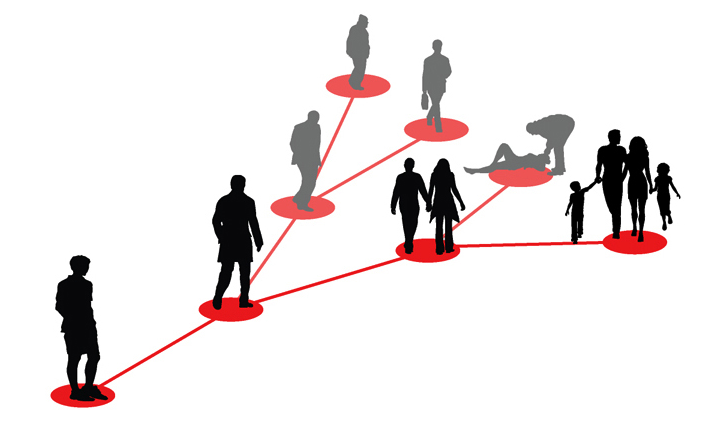
\includegraphics[scale=0.15]{many-worlds.png}
\end{center}
\vspace{-0.2cm}
\end{block}

\end{frame}


\begin{frame}{Time branching}
\vspace{-0.2cm}
\begin{center}
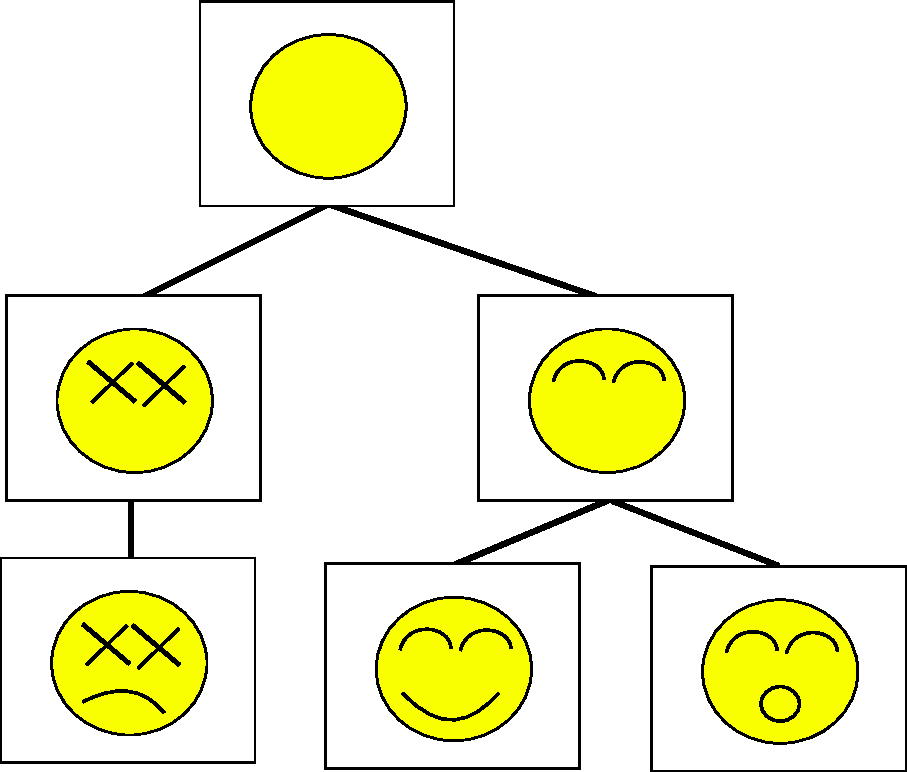
\includegraphics[scale=0.4]{drawing.pdf}\\
\end{center}
\vspace{-0.2cm}
\noindent``Freeze'' a running FRP expression, convert it to a value.\\

Example usages:
\begin{itemize}
\item Duplicate drawing in drawing program into two tabs
\item Undo
\item What-if?
\end{itemize}


\end{frame}

\begin{frame}{Efficiency considerations}
We do not want:

\begin{itemize}
\item Polling \hfill
\includegraphics[scale=0.3]{are-we-there-yet.jpg}
\item Redundant re-evaluations\hfill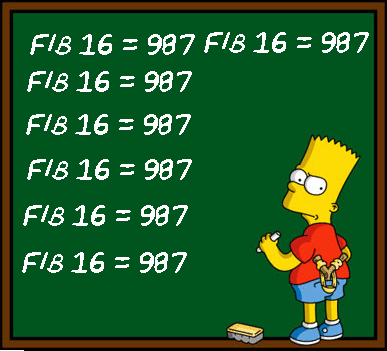
\includegraphics[scale=0.3]{recompute.png}
\end{itemize}

\end{frame}

\begin{frame}{Single future evaluation mechanisms}

\begin{tabular}{l l}
&\emph{Evaluation mechanism} \\
\hline
Reactive & Push-pull \\
FrTime, Scala.React & Self-adjusting computation \\
\end{tabular}\\
\vspace{0.2cm}
Both efficient: prevent polling \& redundant re-evaluations
\end{frame}

\begin{frame}{Time branching evaluation mechanisms}
\begin{tabular}{l l}
 & \emph{Evaluation mechanism}  \\
\hline
Yampa & Continuation based + GADT-based optimizations  \\
\end{tabular}\\
\vspace{0.2cm}
Not as efficient as single future mechanisms: 
\begin{itemize}
\item Does not prevent polling
\item Prevents a large class, but not all, redundant re-evaluations
\end{itemize}
\end{frame}
\section{Solution}

\begin{frame}{Monadic FRP}

We introduce Monadic Functional Reactive Programming.
\begin{itemize}
\item A new programming interface for time-branching  FRP
\item \emph{This talk:} Efficient evaluation mechanism for time-branching FRP: \\
 Continuation based + event requests\\
Prevents:
\begin{itemize}
\item Polling
\item Redundant re-evaluations
\end{itemize}
\end{itemize}
\end{frame}

\newlength{\tmathindenta}
\setlength{\tmathindenta}{\mathindent}
\setlength{\mathindent}{0.05cm}


\begin{frame}{Reactive computations}

\begin{block}{Reactive computation}
A monadic computation which may require the occurrence of external events to continue
\end{block}

All Monadic FRP expressions are built using:
  \begin{itemize}
    \item Basic events :  \\
% spacing!
  Example: |mouseDown :: React GUIEv Int|
    \item Sequential composition:\\ 
 \begin{code}
    (>>=) :: React e a -> (a -> React e b) -> React e b
  \end{code}
\item Parallel composition:  \\
 \begin{code}
 first :: React e a -> React e b -> React e (React e a, React e b)
\end{code}
\end{itemize}

\end{frame}



\begin{frame}{Signal computation}
\begin{block}{Signal computation}
A reactive computation that may also \alert{emit} values.\\
 Defined in terms of reactive computations.
\end{block}
\begin{code}
instance Monad (Sig e f) where ...
waitFor   :: React e r -> Sig e f r
emit      :: f -> Sig e f ()
\end{code}

\end{frame}


\begin{frame}{Signal computation example}

\begin{block}{Example}
\vspace{-0.4cm}
\begin{center}
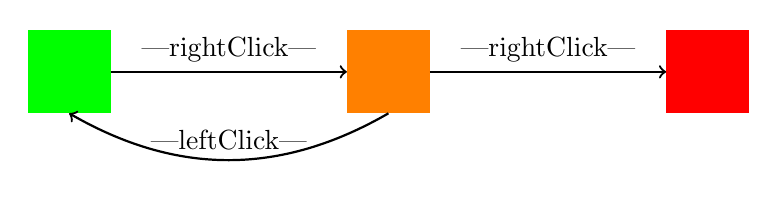
\begin{tikzpicture}[node distance=3cm]
\tikzset{VertexStyle/.style = {shape          = rectangle,
                                 inner sep      = 2pt,
                                 outer sep      = 0pt,
                                 minimum size   = 30 pt}}
     \node[VertexStyle,fill=green](G){};
     \node[VertexStyle,fill=orange,right=of G](OR){};
     \node[VertexStyle,fill=red,right=of OR](R){};   
     %\draw[EdgeStyle](B) to node[LabelStyle]{1} (D) ;
     %\tikzset{EdgeStyle/.append style = {bend left}}
     \draw[thick,->](G) to node[above]{|rightClick|} (OR);
     \draw[thick,->](OR) to node[above]{|rightClick|} (R);
     \draw[thick,->,bend left](OR.south) to node[above]{|leftClick|} (G.south);

  \end{tikzpicture}
\end{center}
\vspace{-0.6cm}
\begin{code}
traffic :: Sig GUIEv Color Void
traffic = 
  do  emit green 
      waitFor rightClick
      emit orange
      (r,_) <- waitFor (rightClick `first` leftClick)
      if done r 
      then  emit red >> waitFor hellFreezesOver 
      else  traffic
\end{code}
\setlength{\mathindent}{\tmathindenta}
\vspace{-0.8cm}
\end{block}
\end{frame}

\begin{frame}{Idea for efficient evaluation}

\begin{block}{Continuation based evaluation}

\begin{code}
data React e a = Done a | Later (e -> React e a) 
\end{code}
We do not know if an event will have any effect.
\end{block}

\begin{block}{Continuation based + requests}
\begin{code}
data React e a = Done a | Later (Requests e) (e -> React e a) 
\end{code}
Add which events the reactive computation \alert{requests}\\ (i.e. is interested in).
\end{block}
\end{frame}

\begin{frame}{Interpreting Monadic FRP expressions}
\begin{block}{Interpret Reactive computation}
Handle event requests in some Monad (for example IO):
\begin{code}
interpret ::  Monad m => (Requests e -> m e) 
              -> React e a -> m a
interpret p (Now a)     = return a
interpret p (Later r c)  = p r >>= interpret p . c
\end{code}
\end{block}

\begin{block}{Interpret Signal computations}
Also handle emissions.
\begin{code}
interpretSig ::  Monad m  => (Requests e -> m e) 
                 -> (a -> m ()) -> Sig e a b -> m b
\end{code}
\end{block}

\end{frame}



\tikzstyle{bag} = [rectangle,text centered,draw=black,semithick,solid]
\tikzstyle{interpret} = [rectangle, rounded corners,text centered,draw=black,semithick]
 \tikzstyle{every node}=[font=\small]

\begin{frame}{Event requests propagate upwards}

\begin{center}
\begin{tikzpicture}[grow=down, level distance=60pt]
[-]

\node[bag, name=root] {|first|}
  [sibling distance=5cm]
  child {node[bag] {|first|}[sibling distance=2.5cm]
    child {node[bag] {|mouseMove|}
       edge from parent[<-]
       node[xshift=-15pt,midway,fill=white,color=white,text=black]{$\{\mathit{MouseMove}\}$}
    }
    child {node[bag] {|mouseUp|}
       edge from parent[<-]
       node[xshift=+15pt,midway,fill=white,color=white,text=black]{$\{\mathit{MouseUp}\}$}
    }
       edge from parent[<-]
       node[xshift=-15pt,midway,fill=white,color=white,text=black]{$\{\mathit{MouseMove},\mathit{MouseUp}\}$}
       %node[left]{$\{\mathit{MouseMove},$ \\ $\mathit{MouseUp}\}$}
  }
   child {node[bag] {|>>=|}  [sibling distance=2.5cm]
child {node[bag] {|mouseDown|}
       edge from parent[<-]
       node[midway,fill=white,color=white,text=black]{$\{\mathit{MouseDown}\}$}
    }
    child {node[bag] {|\ _ -> deltaTime|}
       edge from parent[-]
    }
       edge from parent[<-]
       node[xshift=+15pt,midway,fill=white,color=white,text=black]{$\{\mathit{MouseDown}\}$}
  }
 
 ;
\node[interpret,above of=root,yshift=+20pt,name=inter,text width=3cm] {|interpret|};
\draw [->] (root) --  (inter) node[midway,fill=white,color=white,text=black]{$\{\mathit{MouseMove},\mathit{MouseUp}, \mathit{MouseDown}\}$};
\end{tikzpicture} 
\begin{code}
first (first mouseMove mouseUp) (mouseDown >> deltaTime) 
\end{code}
\end{center}
\end{frame}

\begin{frame}{Set of event requests $\rightarrow$ No polling}

The reactive computation requests an events from the set:
$$\{\mathit{MouseMove},\mathit{MouseUp}, \mathit{MouseDown}\}$$

This is passed to the function |p|, which handles event requests.


\begin{code}
interpret ::  Monad m => (Requests e -> m e) 
              -> React e a -> m a
interpret p (Now a)     = return a
interpret p (Later r c)  = p r >>= interpret p . c
\end{code}

This function can \alert{block} until such an event arrives.

\end{frame}


\begin{frame}{Events propagate downwards: no redundant re-evalutions}
\begin{center}
\begin{tikzpicture}[grow=down, level distance=60pt]
[-]

\node[bag, name=root] {|first|}
  [sibling distance=5cm]
  child {node[bag] {|first|}[sibling distance=2.5cm]
    child {node[bag] {|mouseMove|}
       edge from parent[-,dashed]
    }
    child {node[bag] {|mouseUp|}
       edge from parent[-,dashed]
    }
       edge from parent[-,dashed]
       node[xshift=-15pt,midway,fill=white,color=white,text=black]{$\{\mathit{MouseMove},\mathit{MouseUp}\}$}
  }
   child {node[bag] {|>>=|}  [sibling distance=2.5cm]
child {node[bag] {|mouseDown|}
       edge from parent[red,->,thick]
       node[midway,fill=white,color=white,text=black]{$\{\mathit{MouseDown}\}$}
    }
    child {node[bag] {|\ _ -> deltaTime|}
       edge from parent[black,-,dashed]
    }
    edge from parent[red,->,thick]
       node[xshift=+15pt,midway,fill=white,color=white,text=black]{$\{\mathit{MouseDown}\}$}
  }
 
 ;
\node[interpret,above of=root,yshift=+20pt,name=inter,text width=3cm] {|interpret|};
\draw [red,<-,thick] (root) --  (inter) node[midway,fill=white,color=white,text=black]{Observed : $\{\mathit{MouseDown}\:\mathit{MLeft}\}$};
\end{tikzpicture}
\begin{code}
first (first mouseMove mouseUp) (mouseDown >> deltaTime) 
\end{code}
\end{center}
\end{frame}

\begin{frame}{Next state}

\begin{center}
\begin{tikzpicture}[grow=down, level distance=60pt]
[-]

\node[bag, name=root] {|first|}
  [sibling distance=5cm]
  child {node[bag] {|first|}[sibling distance=2.5cm]
    child {node[bag] {|mouseMove|}
       edge from parent[<-]
       node[xshift=-15pt,midway,fill=white,color=white,text=black]{$\{\mathit{MouseMove}\}$}
    }
    child {node[bag] {|mouseUp|}
       edge from parent[<-]
       node[xshift=+15pt,midway,fill=white,color=white,text=black]{$\{\mathit{MouseUp}\}$}
    }
       edge from parent[<-]
       node[xshift=-15pt,midway,fill=white,color=white,text=black]{$\{\mathit{MouseMove},\mathit{MouseUp}\}$}
       %node[left]{$\{\mathit{MouseMove},$ \\ $\mathit{MouseUp}\}$}
  }
   child {node[bag] {|deltaTime|}  [sibling distance=2.5cm]
child {node[fill=white,color=white,text=white] {|mouseDown|}
edge from parent[white]
    }
    child {node[fill=white,color=white,text=white] {|\ _ -> deltaTime|}
edge from parent[white]
    }
       edge from parent[<-]
       node[xshift=+15pt,midway,fill=white,color=white,text=black]{$\{\mathit{DeltaTime}\}$}
  }
 
 ;
\node[interpret,above of=root,yshift=+20pt,name=inter,text width=3cm] {|interpret|};
\draw [->] (root) --  (inter) node[midway,fill=white,color=white,text=black]{$\{\mathit{MouseMove},\mathit{MouseUp}, \mathit{DeltaTime}\}$};
\end{tikzpicture} 

\begin{code}
first (first mouseMove mouseUp) deltaTime
\end{code}
\end{center}
\end{frame}

\begin{frame}{Evaluation mechanism summary}
Event requests $\rightarrow$ 
\begin{itemize}
\item No polling because we know which events to wait for.
\item No redundant re-evaluations because we know the event requests of each subexpression.
\end{itemize}

\end{frame}

\begin{frame}{In the paper...}
\begin{itemize}
\item Monadic FRP programming interface.
\item Simple drawing program example.
\item Comparison with other FRP programming interfaces \& evaluation mechanisms.
\item Exact time semantics (|sleep 1.0| occurs strictly before |sleep 1.1|).

\item ... and all the details.
\end{itemize}

\end{frame}

\section{Conclusion}
\begin{frame}{Future work}
Implementation of evaluation mechanism currently relies on \emph{closed} union of possible basic events.\\
Downsides:
\begin{itemize}
\item requires explicit memoization for reactive level sharing.
\item reactive level recursion is (very) problematic.
\end{itemize}
Continuation based + GADT-based optimizations mechanism (Yampa) does not have these problems.\\

\vspace{0.5cm}

Possible solution: Use open union instead.
\end{frame}









\begin{frame}{Conclusion}
\noindent Purely functional evaluation mechanism for time-branching FRP:\\
\hspace{0.5cm}Continuation based + event requests\\
Benefits:
\begin{itemize}
\item No polling
\item No redundant re-evaluations.
\end{itemize}
\pause
Questions?
\end{frame}


\begin{frame}[noframenumbering]{Transformational vs. Reactive}
\begin{block}{Transformational program}
Transforms input into output.\\

Examples:
\begin{itemize}
\item Traditional compiler
\item Long-running scientific computation
\end{itemize}
\end{block}

\begin{block}{Reactive program}
Engages in a dialogue with its environment, responding to events.\\

Examples:
\begin{itemize}
\item IDE
\item Spreadsheet
\item Anything with a GUI
\end{itemize}
\end{block}
\end{frame}


\begin{frame}[noframenumbering]{Why Functional Reactive Programming?}
\begin{block}{Reactive programming means...}
Dealing with external events which may occur in \alert{in any order}.\\
\vspace{0.2cm}
Traditional approaches:\\
\begin{tabular}{l l l l}
  & \emph{Approach} & \emph{Downside}\\
\hline
\inlineitem & Concurrency & non-determinism\\
\inlineitem & Callbacks (observer pattern) & inversion of control \\
\inlineitem & I/O multiplexing & non-composable\\
\end{tabular}
\end{block}

\begin{block}{Functional reactive programming}
is \alert{deterministic}, \alert{composable} and \alert{without inversion of control}.
\end{block}


\end{frame}


\end{document}
